\documentclass[11pt,a4paper]{report}

\ifx\pdftexversion\undefined
  \usepackage[dvips]{graphicx}
\else
  \usepackage[pdftex]{graphicx}
   \DeclareGraphicsRule{*}{mps}{*}{}
\fi

\usepackage{iftex}
\usepackage{color}
\ifPDFTeX
    \usepackage[utf8]{inputenc}
\fi
\usepackage[english]{babel}
\usepackage[english]{tuereport2008}
\usepackage{amsmath}
\usepackage{algorithm}
\usepackage{algpseudocode}
\usepackage[T1]{fontenc}

\graphicspath{{images/}}

\title{Visualizing the Netherlands}
\subtitle{2IV05: Additional component computer graphics}
\author{Michiel Fortuin\\Wouter Lok}
\version{2.0}
\orderissuer{}
\copyholder{}
\administrativeunit{Department of Mathematics and Computer Science}   % insert department name here
\department{Visualization}     % subdepartment, or group
\website{}
\reference{}

\begin{document}
\maketitle

\setcounter{tocdepth}{1}
\tableofcontents

\chapter{Introduction}
This report presents the results of the project “Visualizing the Netherlands” as part of the course “Additional component computer graphics”. The goal of the project was to design and implement a system which is able to visualize the Netherland based on the BAG-extract [1] and other open data sources. The BAG-extract is a data set that contains information on all the buildings and addresses in the Netherlands.
%change reference

Firstly, the report presents the open data sets used, then the requirements and the desired functionality of the system is described. In section 4 the problems and challenges of the project are described shortly. Related work, which helped us solving the project’s challenges, is presented in section 5. In the literature study, methods to construct and visualize large worlds out of large data sets have been researched. Then in section 6, a short analysis of the used data sets is made and the system design and algorithms used are presented. The system uses specific data structures and methods to access the out-of-memory data set. Algorithms to construct and to use these data structures are also presented. Further, in section 7 the results of the implementation of the designed system and algorithms are discussed. Here the implemented system will be tested in various scenarios to see how the system performs. Finally a conclusion on the results is made and possible improvements or extensions on the systems are proposed.

\chapter{Open data sets}
\label{chap:OpenDataSets}
The data required to render the Netherlands have been retrieved from two open data sets. Firstly, the BAG dataset \cite{BAG14} was used to extract all necessary information on buildings and secondly OpenStreetMap (OSM) \cite{OSM14} was used to retrieve information about the landscape.

The BAG (Basisadministratie Adressen en Gebouwen) is a data set which contains all kind of information on almost all the buildings and places in the Netherlands. The BAG is provided by Kadaster, but the content of the BAG is owned by the government of cities and they are also responsible to supply the information to Kadaster. A full extraction of the BAG data set called BAG-extract is freely available at various locations. We retrieved the dataset from the Nationaal georegister \cite{NG14}, a website which contains all kind of geographic open data sources. Our dataset contained a version from Januari 2014 and is 40 gB in total.

All information in the BAG-extract is supplied within xml-files and these files are grouped in multiple categories. Each category contains information on a different object-type. The different object-types are presented in table \ref{Table:ObjectTypesBAG} and a full diagram containing all fields of the objects and connections between object types is presented in appendix \ref{chap:DiagramStructureBAG}. All geometric information in the BAG-extract is presented according to the Geography Markup Language (GML). GML is a standard format of providing geometric information with XML.

\begin{table}
  \centering
  \begin{tabular}{l l}
    \textbf{Object type} & \textbf{Content}     \\ \hline
    Towns & Name, boundaries and status  \\ \hline
    Public spaces & Name of the place  \\ \hline
    Numbering & Addresses of buildings and places  \\ \hline
    Buildings & Building surface geometry, build year and status  \\ \hline
    Residences & Geometric location, surface area and status  \\ \hline
    Berths & Surface geometry and status  \\ \hline
    Other areas & Surface geometry and status \\
  \end{tabular}
  \caption{Object-types of the BAG-extract}
  \label{Table:ObjectTypesBAG}
\end{table}

To be able to process all the data in the BAG, the project NLExtract [4] is used to process all data into a database. A script was created to pre-process the data from the database to simple xml-files, which are used to construct the buildings. The numberings object type are filtered to be able to create a small data set which can be used during development. This way only residences with an address in Eindhoven are selected for the construction of buildings. The surface geometry of buildings and the surface area of residences are used to approximate the height of a building.

OpenStreetmap is a website which can be compared to GoogleMaps. Both systems provide a detailed map of the whole world. In contrast to GoogleMaps however, most information which is shown on OpenStreetMap have been provided by the community. Also, the data generated by the project and which is created by the community is accessible freely. Data acquired from OSM is provided in a raw format. The library OSMSharp [5] is used to read and process all the data from OSM. The elements specified by OSM are presented in table \ref{Table:ObjectTypesOSM}. Our system currently only uses ways and nodes with particular tags to render roads; water areas and some other surface area types. Relations between elementents are ignored.
\begin{table}[h]
    \centering
    \begin{tabular}{c p{10cm}}
       \textbf{Element} &  \textbf{Content}     \\ \hline
      Nodes & Points in space in longitude and latitude  \\ \hline
      Ways & Ordered list on nodes as a (closed) polygon or a polyline describing an area, roads or rivers. Tags are used to specify the type of the way.  \\ \hline
      Relation & Data structure to specify relationship between two or more elements  \\
    \end{tabular}
    \caption{Object-types of the OSM data set}
    \label{Table:ObjectTypesOSM}
\end{table} 
\chapter{Requirements}
\label{chap:Requirements}
The application visualizes the Netherlands on the screen in 3D. All the buildings that are in the data set are being rendered. There are datasets for the whole of the Netherlands. It is possible to fly over an area of the Netherlands and walk through cities. Besides buildings, also roads and ground type (grass, farm land, water and industrial terrain) are rendered.
Because of the immensely huge data set of buildings in the Netherlands, this data set is filtered, preprocessed and saved in an efficient format, so that it can be used by the algorithms to construct the world. OpenStreetMap has data about the streets, ground type and trees. That data set is also used to render the world.

\section{Specification of functionality}
\label{sec:SpecificationOfFunctionality}
The following functionality is implemented in the system.
\begin{itemize}
  \item Read data from the BAG data set.\\
    The BAG data set is quite large. The system needs to be able to read and filter the data from the BAG such that the required data can be retrieved.
  \item Construct buildings from geographic data. \\
    Models of buildings need to be constructed from the data read from the BAG. The model of a building has to be modeled to look like the corresponding real building.
  \item Construct roads and surface area.\\
    To make cities and other areas look like the real world, also roads and surface areas like grass, rivers and lakes can be constructed. These elements can contribute highly to make areas recognizable.
  \item Display the constructed world in 3D in real time.\\
    Since rendering a whole area, like Noord Brabant, can be quite large, an efficient rendering algorithm has to be designed or used so that the application can be rendered in real time.
\end{itemize}
\section{Specification of interaction}
\label{sec:SpecificationOfInteraction}
There are 2 different modes to change the view. The first view is that you fly through and over a city or landscape. In the second view, the camera of the system will be set to a height around 1.75m. That way you see the world as any human would see it as he or she would walk through the city. From the start, the user is able to select a city he or she would like to visit. The user is then placed somewhere above or within the city and is able to go anywhere the user wants. Also the speed in which the user is walking or flying can be configured so that the user is able to walk quickly through the city or is able to fly towards another city.

\section{Specification of presentation}
\label{sec:SpecificationOfPresentation}
The world will be rendered dependent on the position of the user. If the user is inside a city, then all buildings in the proximity of the user will be rendered with high detail. While flying the user is able to go to a higher altitude. Since buildings and other parts will become very small, a lower level of detail can be applied to the elements which have to be rendered. When the user gets even higher then multiple buildings will be combined into one model. At the top level, only the landscape will be rendered.
\chapter{Problem description}
The main problem with this project is that the amount of data from the BAG and OpenStreetMap that has to be rendered is larger than the amount of memory available. Also amount of processing power needed to render all the models and the terrain in real-time is too large and is not available in a consumer pc.

\section{Sub problems}
This problem is can be divided in multiple sub problems.
\begin{itemize}
   \item Render less information, without a big concessions on the image quality
   \item Determine what data has to be rendered and what not
   \item Still render the image in real-time
\end{itemize}
Solutions to these problems are presented in section. 
\chapter{Discussion of literature}
\label{chap:DiscussionOfLiterature}
Douglas Davis, William Ribarsky, T.Y. Jiang, Nickolas Faust and Sean Ho \cite{Davis} present a method of rendering large collections of heterogeneous objects. By applying hierarchical paging procedures to terrain and buildings, they are able to visualize out-of-core collections of 3D objects (e.g. cities) in real-time. Further they present a method for efficient handling of culling on large collections of buildings. Finally, the use of level of detail can be incorporated to provide detail management. All of these procedures could be applied to solve part of the main of the problem. 
\chapter{Analysis and solution}
\label{chap:AnalysisAndSolution}
\section{Data analysis}
\label{sec:DataAnalysis}
\subsection{Constructing buildings}
To construct the buildings, we would like to extract data for each building from the BAG data set. However, this data is incomplete. For each building, only a polygon is defined with geographical points. This polygon describes the contour and the exact position of a building. Thus the data contains no information on the height of the building or what kind of roof the building has. In order to determine the height of a building, we can however used the information stored in the residences of a building. For each residence the BAG-dataset contains the total surface area. Combining this with the total area of the surface geometry of a building, we are able to approximate the amount of floors of a building. To approximate the height of a building, we specify that each floor has a height of 2.5 meters. However, for some buildings, only some or no residences are specified, therefore some buildings will get an invalid height. Buildings with no residences will be constructed with an height of 2.5 meters.

Since the bag data set contains no information on the roof, all buildings will get a flat roof. To create the roof for a model cannot be done in a naïve way, since most of the models of the buildings are non-convex polygons. That is, not every point in the polygon is directly visible by all other points, and thus no direct edge can be constructed between two points without the possibility that this edge crosses an edge of the polygon. To produce the roof of a model, an ear slicing algorithm is used. The ear slicing algorithm is a well-known algorithm for triangulating a simple polygon \cite{Kajak11}. The algorithm iteratively locates an ear in the polygon and removes the ear. This process continues till the polygon is a triangle.

A vertex $p_i$ in a polygon is called an ear if the diagonal line between the neighbouring vertexes, $(p_{i-1}, p_{i+1})$, lies entirely within the polygon. That is, this diagonal $(p_{i-1}, p_{i+1}$ does not intersect with any other edge of the polygon. When an ear is found, it is removed from the polygon and the diagonal $(p_{i-1}, p_{i+1})$ will be a new edge within the polygon and the diagonal will be saved in a list. In the end, all the diagonals in the list form the triangulating diagonals for the polygon. An example of a valid ear and the result of the ear-slicing algorithm is shown in figure \ref{fig:ear_slicing}
\begin{figure}[htb!]
    \centering
    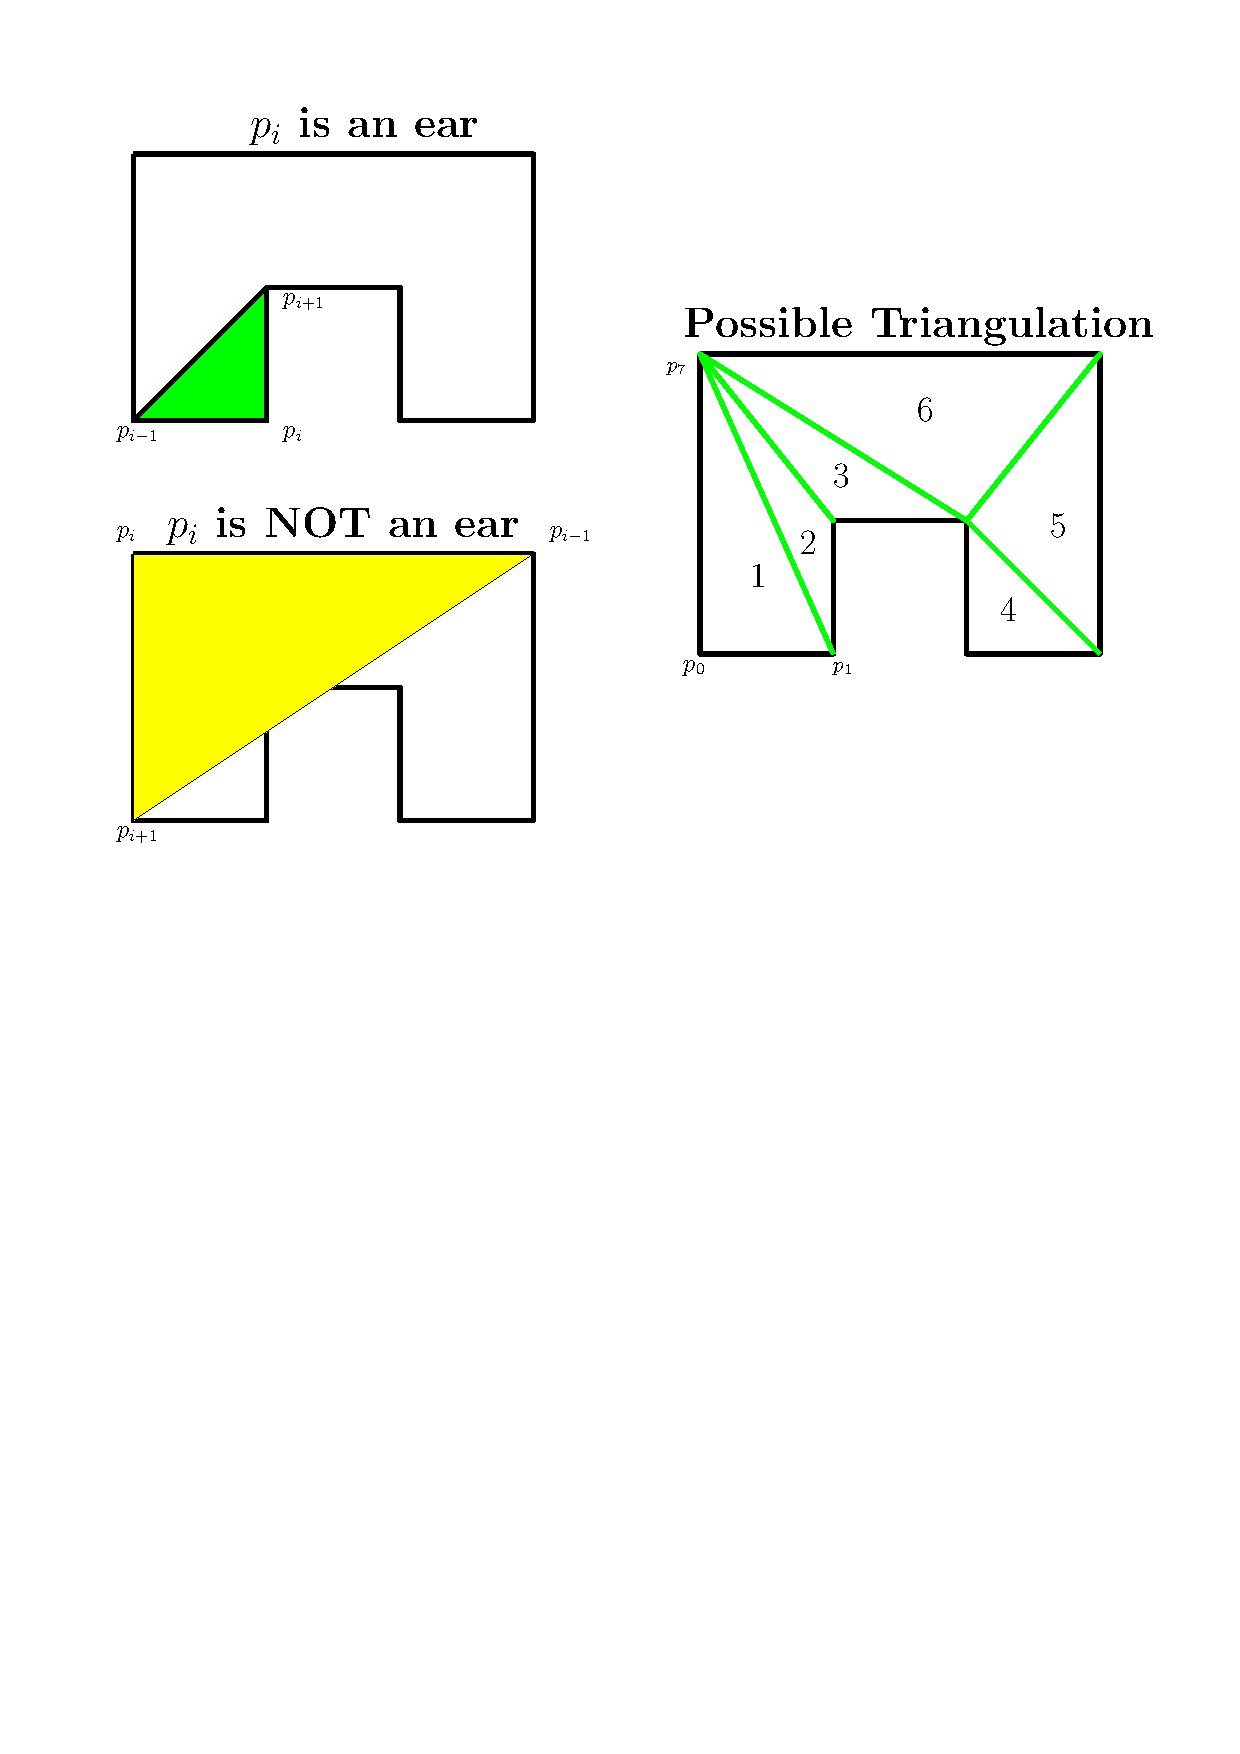
\includegraphics[width=.7\textwidth]{ear_slicing}
    \caption{Example of an ear and ear slicing result}
    \label{fig:ear_slicing}
\end{figure}

\subsection{Constructing roads and surface areas}
We like to use data from OpenStreetMap to construct models of roads, rivers, lakes and other types of surface area. Like described in chapter \ref{chap:OpenDataSets}, a Way in OpenStreetMap describes the position and area of a specific element. Most of Ways also contains a tag. We can use this tag to determine what kind of area the way describes, for example the type of land, water, type of road. If the type is defined in our system, then the system can take the appropriate measures to convert the way into the correct element and apply the corresponding texture. Furthermore, ways can contain meta-information. For example, roads may contain information about the number of lanes. We can use this to approximate the width of a road. For every lane 2.5 meter is used.

\section{System Design}
\label{sec:SystemDesign}
The system is divided in three components. A global overview of the total system is given in figure \ref{fig:sys_overview}. The first component pre-processes all the data, such that the required data from the BAG and OSM data set is processed to application specific objects, which then are collected in a single data set. For example, the system can process only the data from Eindhoven and remove any unneeded metadata. The second component is the Tree building system. The tree-builder uses the pre-processed data to generate a hierarchy binary tree in which multiple levels of details of all the models is stored. Details of building and using the tree is given in section \ref{subsec:HLOD}. The final component of the application visualises the world. A node manager is used to determine which nodes in the tree needs the loaded into memory and rendered.
\begin{figure}[htb!]
    \centering
    \ifPDFTeX
        \includegraphics[width=.4\textwidth]{SystemDesign.1}
    \fi
    \caption{System overview}
    \label{fig:sys_overview}
\end{figure}

\section{Algorithms}
\label{sec:Algorithms}
\subsection{HLOD}
\label{subsec:HLOD}
Davis \cite{Davis} used a quad tree data structure to check what information has to be rendered on the screen. The leaf nodes contains the most detailed models. The non-leafs contains the combined area of it's childeren, but have a simplified model of the data. With such a data structure it is possible to render further away with less detail.

\subsubsection{Generating HLOD}
Algorithm \ref{alg:CreatingANode} can generate a tree (Where an element is a Building, Road, Grass or Water). In this project we have used this method from Davis, with a single modification that it is possible to use a binary tree. The main advantage over a binary tree is that the split in data can be easily be made data dependent. It is difficult to determine where the split in a quad tree has to be made. In a binary tree it is a trivial choice, to balance the tree the median is used to split the data.

\begin{algorithm}[h]
\caption{Creating a node}\label{alg:CreatingANode}
\begin{algorithmic}[1]
\Procedure{CreateNode}{$E$}\Comment{E = List with elements}
\If{$\Call{TriangleCount}{E} < max_{Triangles}$}
    \State $\Call{CreateModelData}{E}$
    \State \Return $E$
\Else
    \State $E_{splits}\gets \Call{Split}{E}$ \Comment{Split list in 2 or 4 parts}
    \For{$i \gets 1,n_{splits}$}
        \State $E_{splits}[i] \gets \Call{CreateNode}{E_{splits}[i]}$
        \State $E_{compiledList}.\Call{Add}{E_{splits}[i]}$
    \EndFor
    \State $\Call{SimplifyData}{E_{compiledList}}$
    \State $\Call{CreateModelData}{E_{compiledList}}$
    \State $\Return E_{compiledList}$
\EndIf
\EndProcedure
\end{algorithmic}
\end{algorithm}

To simplify data the application merges the 2 elements together to get a more simplified version of the original. This merged version is then again added to the list to merge even further. This algorithm is described in \ref{alg:SimplifyData}. The skiplist used in this algorithm is an custom implementation, where deletes can be done in constant time when holding a reference to the specified item. Earlier version of algorithm \ref{alg:SimplifyData}, it was a simpler algorithm, but for every iteration of the while loop it took $O(n^2)$ time. The update function searched every time for the 2 closest elements. We improved this by keeping for every element the closest element and only searched for a new one if the combination between 2 elements is removed. Also in previous version of the algorithm it used when initializing the skiplist a simple linear search to find the closest element. Which makes the the function $InitilizeSkipList$ an $O(n^2)$ algorithm. Later we found a algorithm that can find the nearest neighbor in $O(\log{n})$ time, with an initialization of $O(n\log{n})$ time. So then the function can run in $O(n\log{n})$ time. The whole algorithm was improved from $O(n^2)$ initial and $O(n^2)$ for every iteration too $O(n\log{n})$ initial and $O(n)$ for every iteration.

Only models of the same type are merged, so for example only buildings are merged with only buildings. The merge is dependent on the type of the element. Buildings are the only type that can be merged at the moment. They are merged with by taking the convex hull of both buildings. Besides the merging of elements, elements are also removed to speed up the process. Small elements like residential roads besides houses are removed low in the tree and large roads like the highways are only removed high up in the tree. This removal is also element dependent. In the current implementation only roads are removed at certain heights of the tree.

\begin{algorithm}[h]
\caption{Simplify data}\label{alg:SimplifyData}
\begin{algorithmic}[1]
\Procedure{SimplifyData}{$E$} \Comment{E = List with elements}
\State \Call{RemoveElements}{E}
\State $n_{triangles} \gets \Call{TriangleCount}{}$
\State $Skiplist \gets \Call{Create}{Skiplist}$ \Comment{Skip list with tuple of elements, sorted on distance}
\State $\Call{InitilizeSkipList}{Skiplist, E}$
\While{$n_{triangles} >= max_{Triangles}$}
    \State $combination \gets Skiplist.\Call{ExtractMin}{}$
    \State $n_{triangles} = n_{triangles} - combination.first.n_{triangles}$
    \State $n_{triangles} = n_{triangles} - combination.second.n_{triangles}$
    \State $E_{newElement} = \Call{Merge}{combination.first, combination.second}$
    \State $n_{triangles} = n_{triangles} + E_{newElement}.n_{triangles}$
    \State $\Call{UpdateLists}{Skiplist, E, combination, E_{newElement}}$
\EndWhile
\EndProcedure
\Function{RemoveElements}{$E$}
\For{$i \gets n,1$}
    \If{$E[i].\Call{NeedsToRemove}{}$}
        \State $E.Remove(i)$
    \EndIf
\EndFor
\EndFunction
\Function{InitilizeSkipList}{$Skiplist, E$}
\State $\Call{BuildKDTree}{E}$
\For{$i \gets 1,n$}
    \State $E_{closest} \gets \Call{KDTreeNN}{E[i]}$ \Comment{Find Nearest Neighbor}
    \State $Skiplist.\Call{Add}{Tuple<E[i], E_{closest}>}$
\EndFor
\EndFunction
\Function{UpdateLists}{$Skiplist, E, combination, E_{newElement}$}
\State For every element $E_{references}$ in $E$ that references 1 of $combination$ call $SkipList.\Call{Remove}{E_{references}}$
\State $E_{closest} \gets \Call{FindNN}{E, E_{newElement}}$ \Comment{Find Nearest Neighbor}
\State $Skiplist.\Call{Add}{Tuple<E_{newElement}, E_{closest}>}$
\State $E.\Call{Add}{E_{newElement}}$
\EndFunction
\end{algorithmic}
\end{algorithm}

\subsubsection{Rendering with HLOD}
We used algorithm \ref{alg:DeterminLoadList} to determine what nodes has to be loaded and unloaded. The decisions are base on a function named CalculateDistanceError. This function is a simple linear function based on the distance to a specified node. The algorithm only returns the differences from the original loaded list and the new loaded list. Most of the time nodes have to be replaced by another single node (when getting farther from the nodes) or a single node needs to be replaced by multiple nodes (when getting closer to the nodes).

\begin{algorithm}[h]
\caption{Determine replace list - Part 1}\label{alg:DeterminLoadList}
\begin{algorithmic}[1]
\Procedure{DetermineReplaceList}{$S, P$}\Comment{$S$ = Current node, $P$ = Position viewer}
    \State $P_{error} \gets \Call{CalculateDistanceError}{S, P}$
    \If{$P_{error} > MaxDistanceError$} \Comment{Too far from the viewer}
        \State $UnloadList \gets newList$
        \State $\Call{DetermineUnloadList}{S, UnloadList}$
        \If{$n_{UnloadList} > 0$}
            \State $ReplaceList.\Call{Add}{EmptyList, UnloadList}$
        \EndIf
    \ElsIf{$P_{error} < S_{error} \And n_{childeren} > 0$} \Comment{$S_{error}$ is too high, descend to childeren}
        \If{$\Call{IsLoaded}{S}$}
            \State $LoadList \gets newList$
            \For{$i \gets 1,n_{children}$}
                \State $\Call{DetermineLoadListForUnloadingParent}{S_{children}[i], UnloadList}$
            \EndFor
            \State $ReplaceList.\Call{Add}{LoadList, S}$
        \Else
            \For{$i \gets 1,n_{children}$}
                \State $\Call{DetermineReplaceList}{S_{children}[i], P}$
            \EndFor
        \EndIf
    \Else \Comment{Load S}
        \If{$\neg \Call{IsLoaded}{S}$}
            \State $UnloadList \gets newList$
            \For{$i \gets 1,n_{children}$}
                \State $\Call{DetermineUnloadList}{S_{children}[i], UnloadList}$
            \EndFor
            \State $ReplaceList.\Call{Add}{S, UnloadList}$
        \EndIf
    \EndIf
\EndProcedure
\algstore{DeterminLoadList}
\end{algorithmic}
\end{algorithm}

\begin{algorithm}[h]
\caption{Determine load list - Part 2}
\begin{algorithmic}[1]
\algrestore{DeterminLoadList}
\Function{DetermineUnloadList}{$S, UnloadList$}
    \If{$\Call{IsLoaded}{S}$}
        \State $UnloadList.\Call{Add}{S}$
    \EndIf
    \For{$i \gets 1,n_{children}$}
        \State $\Call{DetermineUnloadList}{S_{children}[i], UnloadList}$
    \EndFor
\EndFunction
\Function{DetermineLoadListForUnloadingParent}{$S, P, LoadList, UnloadList$}
    \State $P_{error} \gets \Call{CalculateDistanceError}{S, P}$
    \If{$P_{error} > MaxDistanceError$} \Comment{Too far from the viewer}
        \State \Call{DetermineUnloadListForError}{S, UnloadList}
    \ElsIf{$P_{error} < S_{error} \And n_{childeren} > 0$} \Comment{$S_{error}$ is too high, descend to childeren}
        \For{$i \gets 1,n_{children}$}
            \State $\Call{DetermineLoadListForUnloadingParent}{S_{children}[i], P, LoadList, UnloadList}$
        \EndFor
    \Else
        \State $LoadList.\Call{Add}{S}$
    \EndIf
\EndFunction
\end{algorithmic}
\end{algorithm}

Besides the algorithm to determine what has to be loaded, a second algorithm is added that loads the specific nodes. Our fist implementation was a simple version that loads everything in the diff lists, then replaces it with its unloading counterparts, and after that unloads the nodes. This became a problem because, when the list is very long it took a while to load everything. Our second implementation is described in \ref{alg:LoadNode}. This algorithm is run until it doesn't doesn't change the loaded list. In this algorithm we check what has to be loaded and then load only the closest element. This way if loading takes a bit longer than expected, the position is updated while loading the element. For instance if the application is loading Amsterdam, and the user wants to jump to Eindhoven, it isn't still loading Amsterdam, but starts immediately loading Eindhoven. If nodes are only unloaded and not replaced by anything, this can happen if the node is to far from the viewpoint, then it unloads immediately. Unloading can almost be done instantly, so this isn't really a performance issue. We have added that part, berceuse the application has a lower memory footprint.

\begin{algorithm}[h]
\caption{Loading closest node}\label{alg:LoadNode}
\begin{algorithmic}[1]
\Procedure{CreateNode}{$root, P$} \Comment{$root$ = root node, $P$ = Position viewer}
    \State $replaceList \gets DetermineReplaceList(root, P)$
    \If{$n_{replaceList} \> 0$}
        \State $replace \gets \Call{FindClosest}{replaceList, P}$
        \For{$i \gets 1,n_{replace.LoadNodes}$}
            \State $\Call{Load}{replace.LoadNodes[i]}$
        \EndFor
        \For{$i \gets 1,n_{replace.UnloadNodes}$}
            \State $\Call{Unload}{replace.UnloadNodes[i]}$
        \EndFor
        
        \For{$i \gets 1,n_{replaceList}$}
            \If{$n_{replaceList.LoadNodes} = 0 \And \neg (replace = replaceList[i])$}
                \For{$j \gets 1,n_{replaceList[i].UnloadNodes}$}
                    \State $\Call{Unload}{replaceList[i].UnloadNodes[j]}$
                \EndFor
            \EndIf
        \EndFor
    \EndIf
\EndProcedure
\end{algorithmic}
\end{algorithm}


\subsection{Complex polygons}
\label{subsec:ComplexPolygons}
The OSM data is built out of GPS recordings and these recordings have a lot of noise. The noise has the possibility of creating complex polygons in the OSM data. A complex polygon is a self-intersecting polygon. In our OSM data set we have detected multiple complex polygons. This is a problem because the ear-clipping algorithm can only be used for simple polygons. A simple polygon is a polygon that does not contain intersecting edges and does not contain any holes. OSM does not contain any polygons with holes. The detection for a self-intersecting polygons is a naïve algorithm. If two non-consecutive line-segments of a polygon intersect, then the polygon is complex.

To generate a set of simple polygons from a complex polygon, the algorithm has to find two line-segments that intersect. The point at which two edges intersect, two new polygons can be generated. These two new polygons can still be a complex polygon, so the algorithm has to be recursively called on these new polygons. If the input polygon is already simple, then it simply returns the input polygon.

\section{Motivation of choices made}
\label{sec:MotivationOfChoicesMade}
\subsection{Simple polygon test}
\label{subsec:SimplePolygonTest}
Testing if a polygon is simple is done in a naïve way, a faster method is for example the Bentley-Ottmann algorithm \cite{Bentley79}. This algorithm has a running time of $O(\frac{n^2}{\log{n}})$, which is faster that our naïve way with running time $O(n^2)$. We choose the naïve way, since the polygons in the data set are not very large. The largest polygon in the data set containing only Eindhoven had 60 points. Also the time in which we had to develop the application demanded that we used an algorithm that was relative simple to implement.

\subsection{Simple triangulation}
\label{subsec:SimpleTriangulation}
The ear slicing algorithm implemented also has a running time of $O(n^2)$. There also exist algorithms which can triangulate a polygon in $O(n\log(n))$ and $O(n)$ time. These algorithms are however also more complex to implement. And just like for the simple polygon test, our data set only contains relatively small polygon, therefore the larger complexity does not form a large constraint.

\chapter{Results and evaluation}
\section{Image results}
%todo add images
Figure 1 shows the centre of Eindhoven. This is a basic view of the city of Eindhoven. In the distance there is also water, this river is called the Dommel. This picture is taken on the 18 September plein.

The error that is introduced when rendering from a distance is visible in figure 2 and figure 3. Figure 2 is rendered with an error rate of 100 per meter. Figure 3 is rendered without any error. There are small differences between the images. When looking at the buildings in the bottom and the right of the image, it can be seen that some buildings have been simplified.

\section{GPU usage}
We have tested our system with 2 versions of the data set. The first data set is a single node tree with whole Eindhoven in this single node, thus only the highest level of detail is used. So the visualize application can only render the single node. The second version was a set where Eindhoven was divided in the tree, so the visualize application could choose which nodes it can render. Also in the second version, the error per meter was set on 500.

figure 4 shows the GPU (Graphics Processing Unit) load for the 2 tests and also what the GPU load is when the application isn’t running. When running the test with a single node the GPU load is a lot higher than for the multi node test.

figure 5 presents the memory usage on the GPU for the 2 tests and also shows the memory usage when the application isn’t running. The single node dataset uses a bit more memory than the multi node dataset. Also when the application doesn’t run, the system also uses video memory.

\section{Limitations}
The height of buildings is determined with the building surface area of the building. If the building has an underground structure like underground parking garage, then the building is extremely high. The surface area of the geographic polygon is very small against the surface area of the whole building. This limitation expresses itself by generating very high building, while in reality the building above the ground is very low.

The width of a road is also approximated, by using meta-data. Sometimes this metadata isn’t available or wrong, which results in a different width. Also the road could have wider or smaller lanes.


\chapter{Conclusion and future work}
Our application can successfully render every building from Eindhoven, every element with grass and water and the roads. The objects have textures drawn on them to look appealing. Also different kinds of roads have different textures. The Buildings are generated from the BAG dataset and the other elements are generated from OpenStreetMap data set.

The data is rendered in real-time. Our tests show that a HLOD can make a big difference in rendering this kind of data. The GPU load is about 1.7 times lower with some error introduced, while the differences are not visible on the screen. The memory difference isn’t great. We assume that this is because the data set is relative small. Our single node data set is only 170MB. When the size increases, then the dataset does not fit in the GPU memory and then it will probably show that the memory usage is still very low.

The error that we introduce, which causes simplified versions of buildings to be rendered, is visible in some cases. This is only so little that most of the time this is unnoticeable. When there is a lot of occlusion then this error can even be increased, so the GPU has even less work.

The application can be improved by an algorithm that gives better result when simplifying the models. Also more data can be imported from OpenStreetMap. At the moment, all of our buildings have the same texture. The visualisation can be made even more appealing by applying different textures to buildings. This could be done based on the type of a building and the build year. Also more functionality could be introduced. Now, users can only fly or walk through the world to see what it looks like. The possibility to get information on buildings and the surrounding area would make the application more interesting.

\chapter{Bibliography}
\label{chap:Bibliography}
\begingroup
\renewcommand{\chapter}[2]{}% for other classes
\begin{thebibliography}{}
\bibitem{BAG14}
"BAG-Extract," Kadaster, [Online]. Available: http://www.kadaster.nl/web/artikel/productartikel/BAG-Extract.htm. [Accessed March 2014].
\bibitem{OSM14}
"Open Street Map," [Online]. Available: http://www.openstreetmap.org/about. [Accessed March 2014].
\bibitem{NG14}
"Inspire Adressen," [Online]. Available: http://geodata.nationaalgeoregister.nl/inspireadressen/atom{\slash}inspireadressen.xml. [Accessed February 2014].
\bibitem{NLExtract14}
"NLExtract," opengeogroep, [Online]. Available: https://github.com/opengeogroep/NLExtract. [Accessed February 2014].
\bibitem{OSMSharp14}
"OSMSharp," SharpSoftware, [Online]. Available: http://www.osmsharp.com/. [Accessed March 2014].
\bibitem{Davis}
D. Davis, W. Ribarsky, T. Jiang, N. Faust and a. S. Ho, "Real-Time Visualization of Scalably Large Collections of Heterogeneous Objects".
\bibitem{Kajak11}
B. Kajak, "Improved algorithms for ear-clipping triangulation," 2011.
\bibitem{Bentley79}
J. L. Bentley and T. A. Ottmann, "Algorithms for Reporting and Counting," IEEE TRANSACTIONS ON COMPUTERS,, Vols. c-28, no. 9, pp. 643-647, 1979.
\end{thebibliography}
\endgroup

\appendix
\chapter{Diagram structure BAG}
\label{chap:DiagramStructureBAG}
The diagram below presents the full data specification of the BAG-extract data set. It has been retrieved from the documentation provided by the Kadaster [1].
%add image

\end{document} 